\documentclass[aspectratio=169]{beamer}
\usetheme{UFS}
\usepackage[utf8]{inputenc}
\usepackage[portuguese]{babel}
\usepackage{amsmath,amssymb}
\usepackage{booktabs}
\usepackage{clrscode3e}
\usepackage{xcolor}
\usepackage{graphicx}
\usepackage{tikz}
\usetikzlibrary{shapes.geometric, arrows, positioning, fit, backgrounds, calc, arrows.meta, decorations.pathreplacing}

\graphicspath{{../Figures/Cormen_Ch11/}{../Figures/}}

\definecolor{destaque}{HTML}{E8F5E9}
\definecolor{alerta}{HTML}{FFF3E0}
\definecolor{invariante}{HTML}{E3F2FD}
\definecolor{exercicio}{HTML}{FCE4EC}
\definecolor{slotOcup}{HTML}{C8E6C9}
\definecolor{slotVazio}{HTML}{ECEFF1}
\definecolor{slotColisao}{HTML}{FFCDD2}

\title{Tabelas Hash}
\subtitle{COMP0497 -- Algoritmos e Estrutura de Dados 1}
\author{Prof.\ Dr.\ André Yoshiaki Kashiwabara}
\date{}

% Crédito padrão para as figuras do Cormen
\newcommand{\creditoCormen}{\par\vspace{0.15cm}\scriptsize\itshape Fonte: Cormen, Leiserson, Rivest, Stein --- \emph{Introduction to Algorithms} (2.ed., MIT Press, 2001), Cap.\ 11.}

\begin{document}
\shorthandoff{"}

\begin{frame}
  \titlepage
\end{frame}

\begin{frame}{Roteiro da Aula}
\tableofcontents
\end{frame}

%==============================================================
\section{Motivação: por que precisamos de hash?}
%==============================================================

\begin{frame}{Onde tabelas hash já aparecem no seu dia a dia}
\begin{itemize}
\item \textbf{Python:} todo \texttt{dict} e \texttt{set} é uma tabela hash (CPython usa endereçamento aberto com sondagem perturbada).
\item \textbf{Java:} \texttt{HashMap}, \texttt{HashSet}, \texttt{ConcurrentHashMap} (encadeamento com conversão para árvore quando uma lista cresce demais).
\item \textbf{Bancos de dados:} índices hash, \texttt{GROUP BY}, joins por hash.
\item \textbf{Sistemas:} caches (Redis, Memcached), tabelas de roteamento, deduplicação.
\item \textbf{Compiladores:} tabela de símbolos (variáveis $\to$ tipo, escopo, endereço).
\item \textbf{Bioinformática:} indexar $k$-mers de DNA, busca em genomas.
\item \textbf{Versionamento (Git):} cada objeto é endereçado pelo hash de seu conteúdo.
\end{itemize}
\end{frame}

\begin{frame}[shrink=10]{O problema do dicionário}
\begin{itemize}
\item Queremos uma estrutura que suporte três operações sobre um conjunto dinâmico de chaves:
\begin{itemize}
  \item \textsc{Insert}$(T, x)$
  \item \textsc{Search}$(T, k)$
  \item \textsc{Delete}$(T, x)$
\end{itemize}
\item \textbf{Ideal:} cada uma em $O(1)$ \emph{esperado}.
\end{itemize}
\begin{block}{Comparação rápida}
\centering
\begin{tabular}{lccc}
\toprule
Estrutura & Busca & Inserção & Remoção \\
\midrule
Lista ligada & $\Theta(n)$ & $\Theta(1)$ & $\Theta(n)$ \\
Array ordenado & $\Theta(\log n)$ & $\Theta(n)$ & $\Theta(n)$ \\
Árvore balanceada (AVL, R-B) & $\Theta(\log n)$ & $\Theta(\log n)$ & $\Theta(\log n)$ \\
\textbf{Tabela hash} & $\Theta(1)$ esperado & $\Theta(1)$ esperado & $\Theta(1)$ esperado \\
\bottomrule
\end{tabular}
\end{block}
\end{frame}

\begin{frame}[shrink=10]{Quanto isso importa na prática?}
\textbf{Cenário:} contar palavras distintas em um corpus de $n = 10^7$ palavras.
\centering
\begin{tabular}{lrr}
\toprule
Estrutura & Operações ($\sim n \log n$ ou $n$) & Tempo estimado \\
\midrule
Lista ligada (busca linear) & $\sim 5 \times 10^{13}$ & dias \\
Árvore balanceada & $\sim 2{,}3 \times 10^8$ & $\sim 5$ s \\
Tabela hash & $\sim 10^7$ & $\sim 0{,}1$ s \\
\bottomrule
\end{tabular}

\vspace{0.4cm}
\begin{itemize}
\item Hash não é mais rápido por mágica: ele \emph{evita comparar chaves} ao calcular o endereço diretamente.
\item Preço: precisamos pensar em \alert{colisões} (duas chaves caem no mesmo slot).
\item Garantia é em \emph{expectativa}, não em pior caso (exceto hashing perfeito).
\end{itemize}
\end{frame}

\begin{frame}{Exemplo prático: tabela de símbolos do compilador}
\begin{itemize}
\item Um compilador precisa associar nomes de variáveis (\texttt{contador}, \texttt{idade}, \texttt{x}) a informações (tipo, escopo, endereço).
\item São poucos identificadores ativos por vez (digamos, $10^4$), porém o \emph{universo} possível é gigantesco: todas as strings ASCII de até 30 caracteres $\Rightarrow$ $\sim 128^{30}$.
\item Não dá para reservar memória para cada string possível.
\item \alert{Solução:} converter cada chave em um índice de um array pequeno via uma \emph{função hash}.
\end{itemize}
\begin{exampleblock}{Intuição}
A função hash funciona como o cadastro do CPF em uma fila do banco: o número do CPF tem 11 dígitos, mas o sistema usa apenas os \emph{últimos dois} para distribuir clientes em 100 guichês.
\end{exampleblock}
\end{frame}

%==============================================================
\section{Tabelas de Endereçamento Direto}
%==============================================================

\begin{frame}{Endereçamento direto: a ideia mais simples}
\begin{columns}[T]
\begin{column}{0.55\textwidth}
\begin{itemize}
\item Suponha que o universo $U = \{0, 1, \dots, m-1\}$ é \alert{pequeno}.
\item Usamos um array $T[0\,..\,m-1]$ tal que
$$T[k] = \begin{cases} x, & \text{se } x.\textit{key} = k \\ \textsc{nil}, & \text{caso contrário} \end{cases}$$
\item Todas as operações são $\Theta(1)$ \emph{garantido}.
\end{itemize}
\end{column}
\begin{column}{0.45\textwidth}
\centering
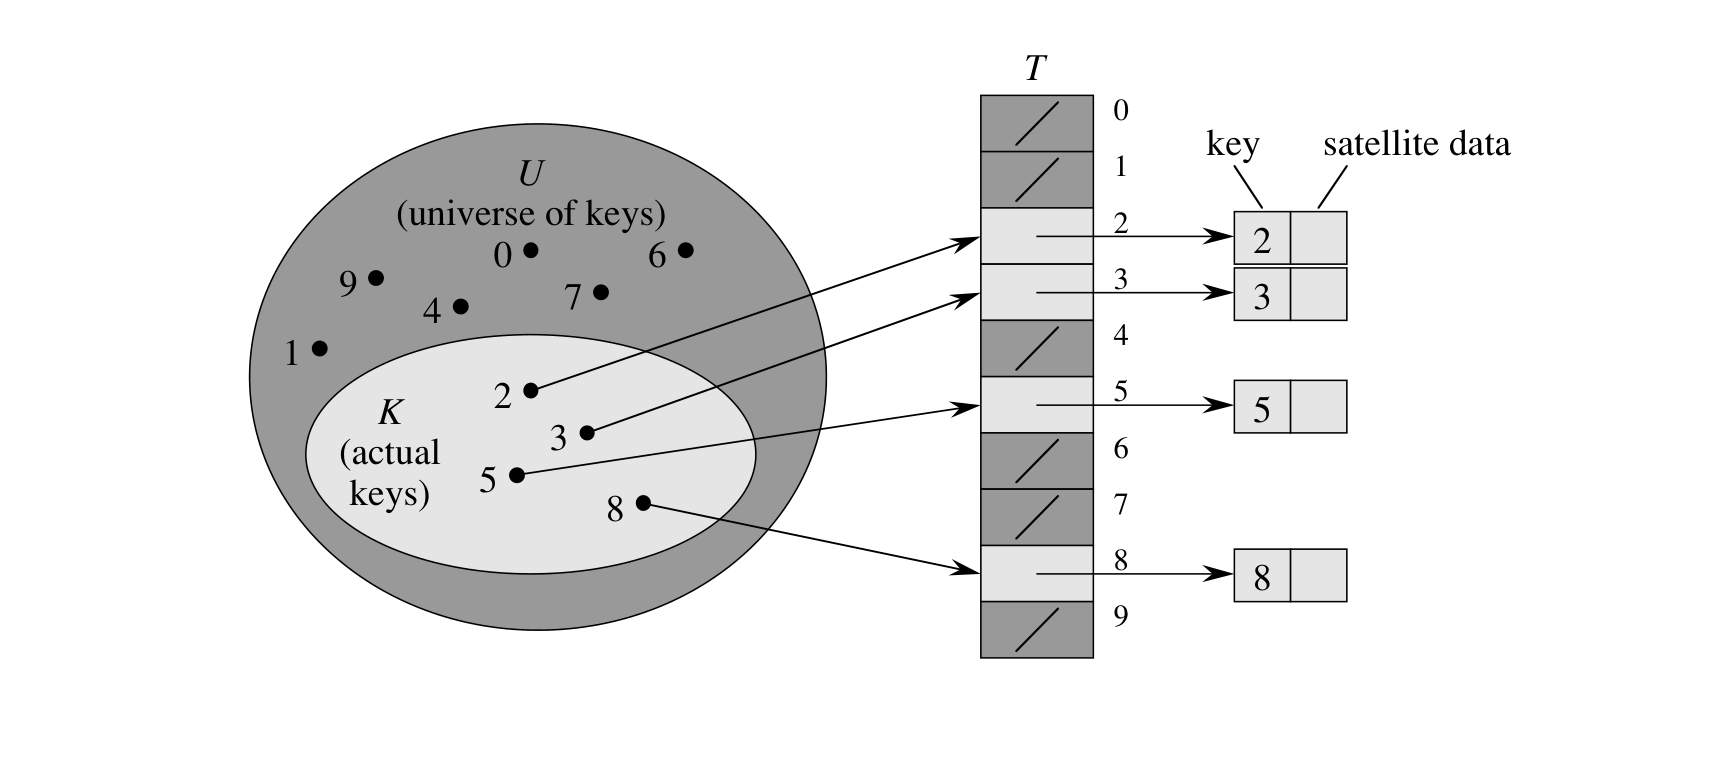
\includegraphics[width=\linewidth]{fig_11_1.png}
{\scriptsize Endereçamento direto.}
\end{column}
\end{columns}
\end{frame}

\begin{frame}[fragile]{Operações de endereçamento direto}
\begin{columns}[T]
\begin{column}{0.32\textwidth}
\begin{codebox}
\Procname{$\proc{Direct-Address-Search}(T,k)$}
\li \Return $T[k]$
\end{codebox}
\end{column}
\begin{column}{0.32\textwidth}
\begin{codebox}
\Procname{$\proc{Direct-Address-Insert}(T,x)$}
\li $T[x.\textit{key}] \gets x$
\end{codebox}
\end{column}
\begin{column}{0.32\textwidth}
\begin{codebox}
\Procname{$\proc{Direct-Address-Delete}(T,x)$}
\li $T[x.\textit{key}] \gets \const{nil}$
\end{codebox}
\end{column}
\end{columns}

\vspace{0.5cm}
\begin{alertblock}{Quando \emph{não} funciona}
Se $|U|$ é enorme (ex.: chaves de 64 bits $\Rightarrow$ $2^{64}$ posições), o array é inviável. E se $|K| \ll |U|$ (poucas chaves ativas), o espaço é quase todo desperdiçado.
\end{alertblock}
\end{frame}

%==============================================================
\section{Tabelas Hash com Encadeamento}
%==============================================================

\begin{frame}{Da tabela direta para a tabela hash}
\begin{columns}[T]
\begin{column}{0.50\textwidth}
\begin{itemize}
\item \alert{Ideia:} use um array $T[0\,..\,m-1]$ com $m \ll |U|$.
\item Uma \textbf{função hash} $h : U \to \{0, 1, \dots, m-1\}$ comprime chaves em índices.
\item Dizemos que ``$k$ \emph{hash-eia} no slot $h(k)$''.
\item Inevitavelmente, $h(k_2) = h(k_5)$ para chaves distintas $\Rightarrow$ \alert{colisão}.
\end{itemize}
\end{column}
\begin{column}{0.50\textwidth}
\centering
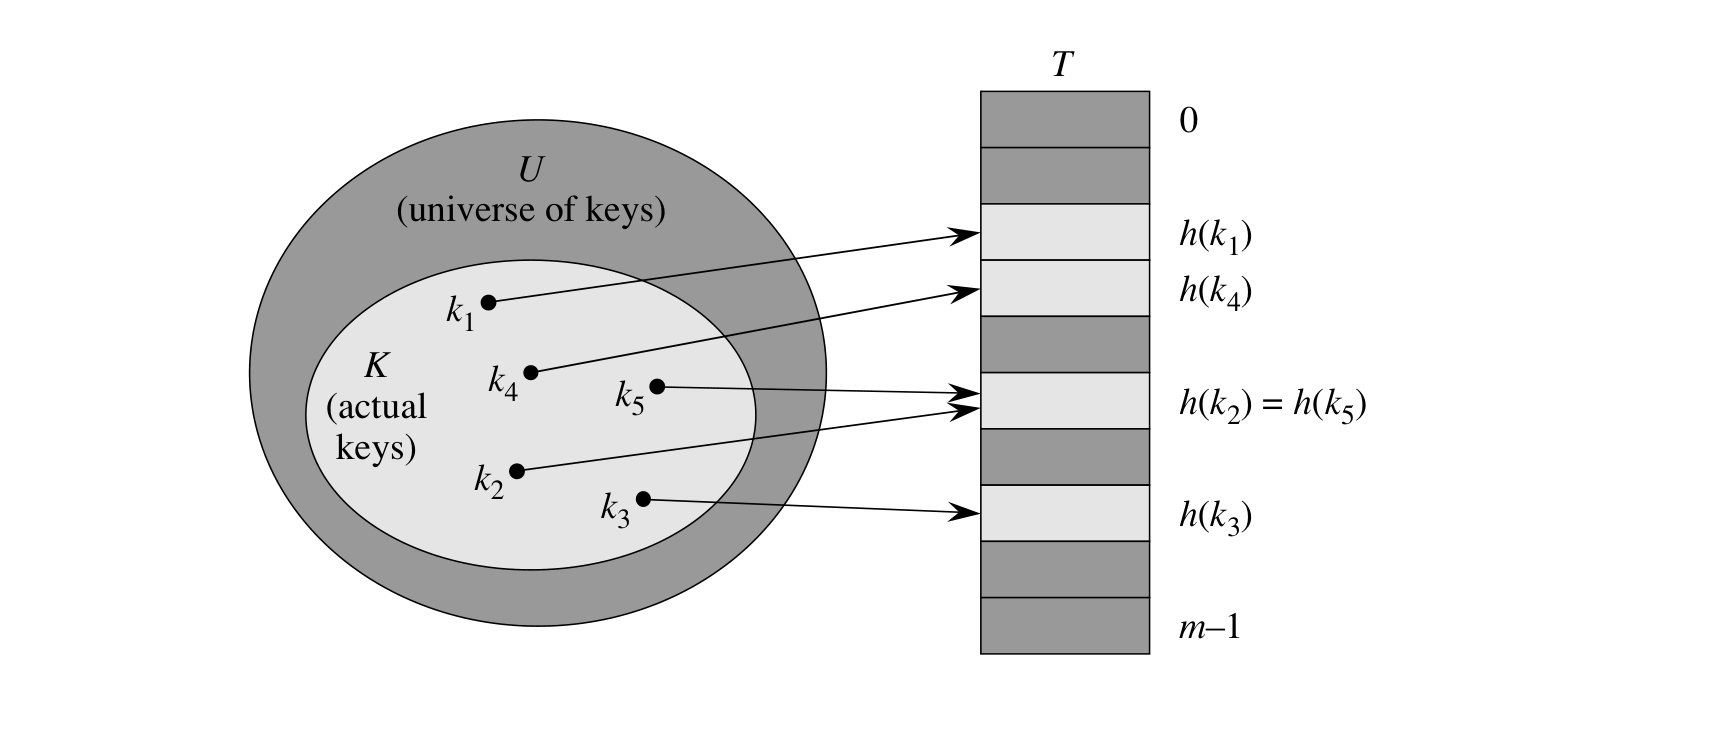
\includegraphics[width=\linewidth]{fig_11_2.png}
{\scriptsize Função hash $h$ mapeia $U$ em $m$ slots.}
\end{column}
\end{columns}
\end{frame}

\begin{frame}{Resolução de colisões por encadeamento}
\begin{columns}[T]
\begin{column}{0.55\textwidth}
\begin{itemize}
\item Cada slot $T[j]$ guarda o \emph{cabeça} de uma lista ligada.
\item Todas as chaves que hash-eiam em $j$ vão para a lista $T[j]$.
\item Operações:
  \begin{itemize}
  \item Inserção: $O(1)$ (insere no início da lista).
  \item Busca: proporcional ao comprimento da lista.
  \item Remoção: $O(1)$ com lista duplamente ligada.
  \end{itemize}
\end{itemize}
\end{column}
\begin{column}{0.45\textwidth}
\centering
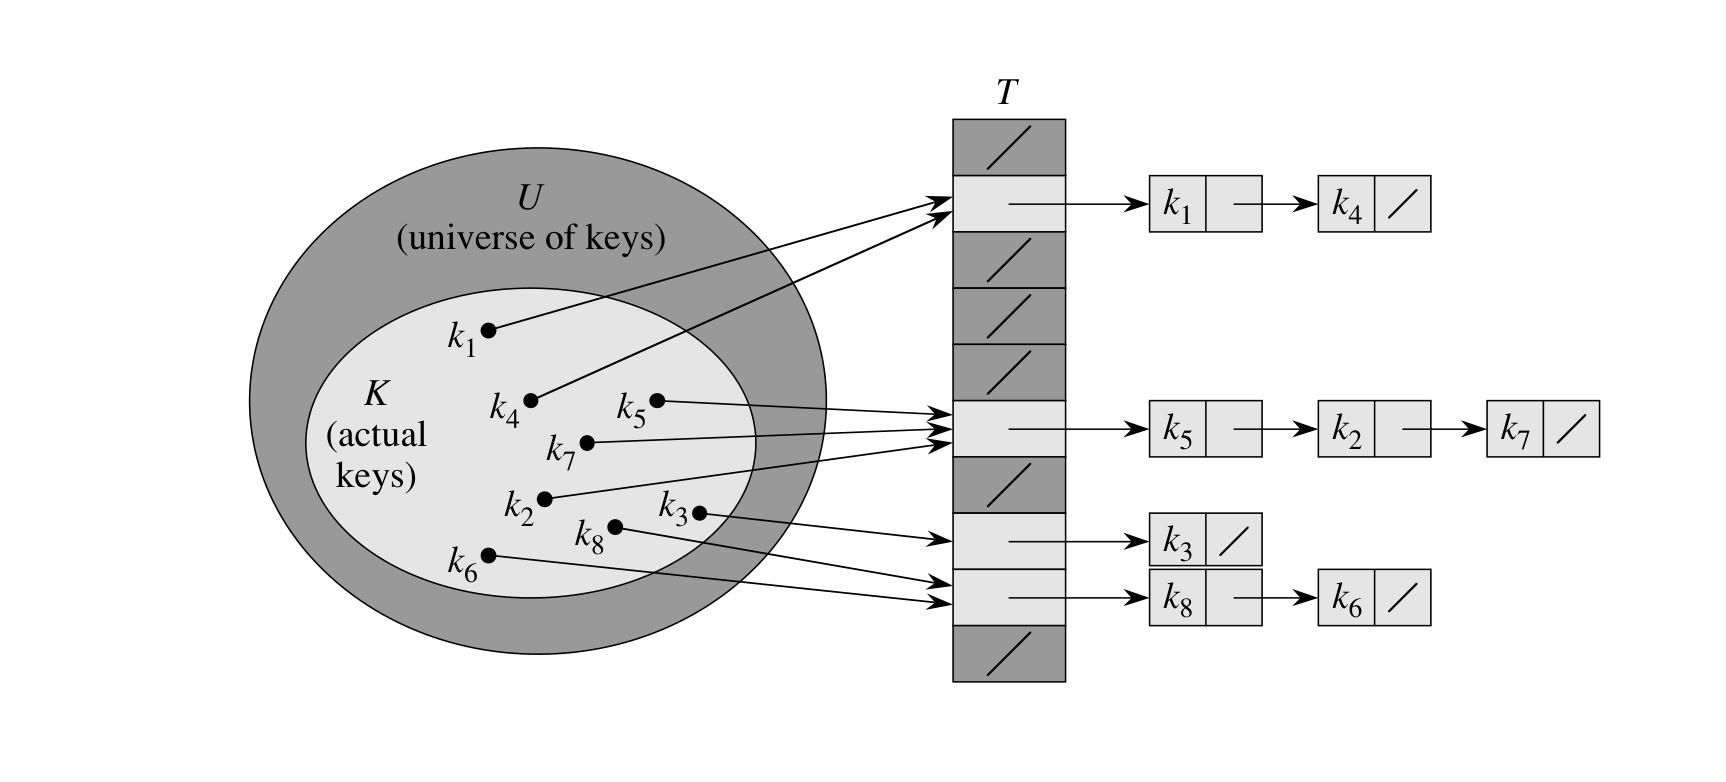
\includegraphics[width=\linewidth]{fig_11_3.png}
{\scriptsize Encadeamento: cada slot aponta para uma lista.}
\end{column}
\end{columns}
\end{frame}

\begin{frame}{Exemplo trabalhado: encadeamento passo a passo}
\textbf{Dados:} $m = 7$, $h(k) = k \bmod 7$. Inserir $50, 700, 76, 85, 92, 73, 101$.

\smallskip
\centering
\begin{tabular}{rcl}
\toprule
$k$ & $k \bmod 7$ & vai para o slot \\
\midrule
50 & $50 = 7\cdot 7 + 1$ & 1 \\
700 & $700 = 7\cdot 100 + 0$ & 0 \\
76 & $76 = 7\cdot 10 + 6$ & 6 \\
85 & $85 = 7\cdot 12 + 1$ & 1 \quad(colisão com 50) \\
92 & $92 = 7\cdot 13 + 1$ & 1 \quad(colisão com 50, 85) \\
73 & $73 = 7\cdot 10 + 3$ & 3 \\
101 & $101 = 7\cdot 14 + 3$ & 3 \quad(colisão com 73) \\
\bottomrule
\end{tabular}

\smallskip
\textbf{Resultado:} listas $T[0]=[700]$, $T[1]=[92, 85, 50]$, $T[3]=[101, 73]$, $T[6]=[76]$.\\
Comprimento médio $= 7/7 = 1$ $\Rightarrow$ $\alpha = 1$. Buscas custam em média $\Theta(2)$.
\end{frame}

\begin{frame}[shrink=10]{Análise: fator de carga}
\begin{block}{Definição: fator de carga $\alpha$}
Para uma tabela $T$ com $m$ slots armazenando $n$ chaves, definimos
$$\alpha = \frac{n}{m}.$$
$\alpha$ é o \emph{comprimento médio} de uma lista no encadeamento.
\end{block}
\textbf{Hipótese de hashing uniforme simples:} cada chave tem probabilidade $1/m$ de cair em qualquer slot, independentemente das outras.

\medskip
\textbf{Teorema (11.1--11.2 do Cormen):} sob hashing uniforme simples, uma busca (com ou sem sucesso) leva em média
$$\Theta(1 + \alpha).$$
Se $n = O(m)$, então $\alpha = O(1)$ e a busca é $\Theta(1)$ em média.
\end{frame}

%==============================================================
\section{Funções Hash}
%==============================================================

\begin{frame}{O que faz uma boa função hash?}
\begin{itemize}
\item \textbf{Determinística:} a mesma chave sempre vai ao mesmo slot.
\item \textbf{Computável rapidamente:} idealmente $O(1)$.
\item \textbf{Distribuição uniforme:} aproxima a hipótese de hashing uniforme.
\item \textbf{Independente de padrões nas chaves:} chaves parecidas (\texttt{x1}, \texttt{x2}, \texttt{x3}) devem ir a slots diferentes.
\end{itemize}
\begin{alertblock}{Não confunda}
Função hash $\neq$ função hash \emph{criptográfica} (SHA-256, etc.). Para tabelas hash queremos velocidade e boa distribuição estatística, não resistência a adversários.
\end{alertblock}
\end{frame}

\begin{frame}{Método da divisão}
\begin{block}{Fórmula}
$$h(k) = k \bmod m$$
\end{block}
\begin{itemize}
\item Simples e rápido (um único \texttt{mod}).
\item Escolha de $m$ é crítica:
\begin{itemize}
\item Evitar $m = 2^p$: $h(k)$ pega só os $p$ bits menos significativos de $k$, descartando o resto.
\item \alert{Boa prática:} $m$ primo, distante de potências de $2$ e de $10$.
\end{itemize}
\item Exemplo: para $n = 2000$ chaves com $\alpha \approx 3$, escolha $m = 701$ (primo perto de $2000/3$).
\end{itemize}
\end{frame}

\begin{frame}[shrink=20]{Por que $m = 2^p$ é ruim?}
\textbf{Exemplo:} $m = 8 = 2^3$, $h(k) = k \bmod 8$.

\smallskip
Considere chaves cujos $3$ bits menos significativos são todos iguais:
\centering
\begin{tabular}{rrll}
\toprule
$k$ & binário & $k \bmod 8$ & slot \\
\midrule
8 & $0000\,1\underline{000}$ & 0 & 0 \\
16 & $0001\,0\underline{000}$ & 0 & 0 \\
24 & $0001\,1\underline{000}$ & 0 & 0 \\
32 & $0010\,0\underline{000}$ & 0 & 0 \\
\bottomrule
\end{tabular}

\smallskip
\alert{Todas no mesmo slot.} A função descartou $|k|/8$ bits de informação.

\smallskip
\textbf{Com $m = 7$ (primo):}
\centering
\begin{tabular}{rcc}
\toprule
$k$ & $k \bmod 7$ & slot \\
\midrule
8 & 1 & 1 \\
16 & 2 & 2 \\
24 & 3 & 3 \\
32 & 4 & 4 \\
\bottomrule
\end{tabular}
\end{frame}

\begin{frame}{Método da multiplicação}
\begin{columns}[T]
\begin{column}{0.55\textwidth}
\begin{block}{Fórmula}
$$h(k) = \lfloor\, m\, (k A \bmod 1)\,\rfloor, \quad 0 < A < 1.$$
\end{block}
\begin{itemize}
\item Vantagem: o valor de $m$ \emph{não é crítico} (qualquer potência de 2 serve).
\item Knuth sugere $A \approx (\sqrt{5}-1)/2 \approx 0{,}6180\dots$ (razão áurea).
\item Implementação eficiente em palavras de $w$ bits: multiplicar e extrair $p$ bits.
\end{itemize}
\end{column}
\begin{column}{0.45\textwidth}
\centering
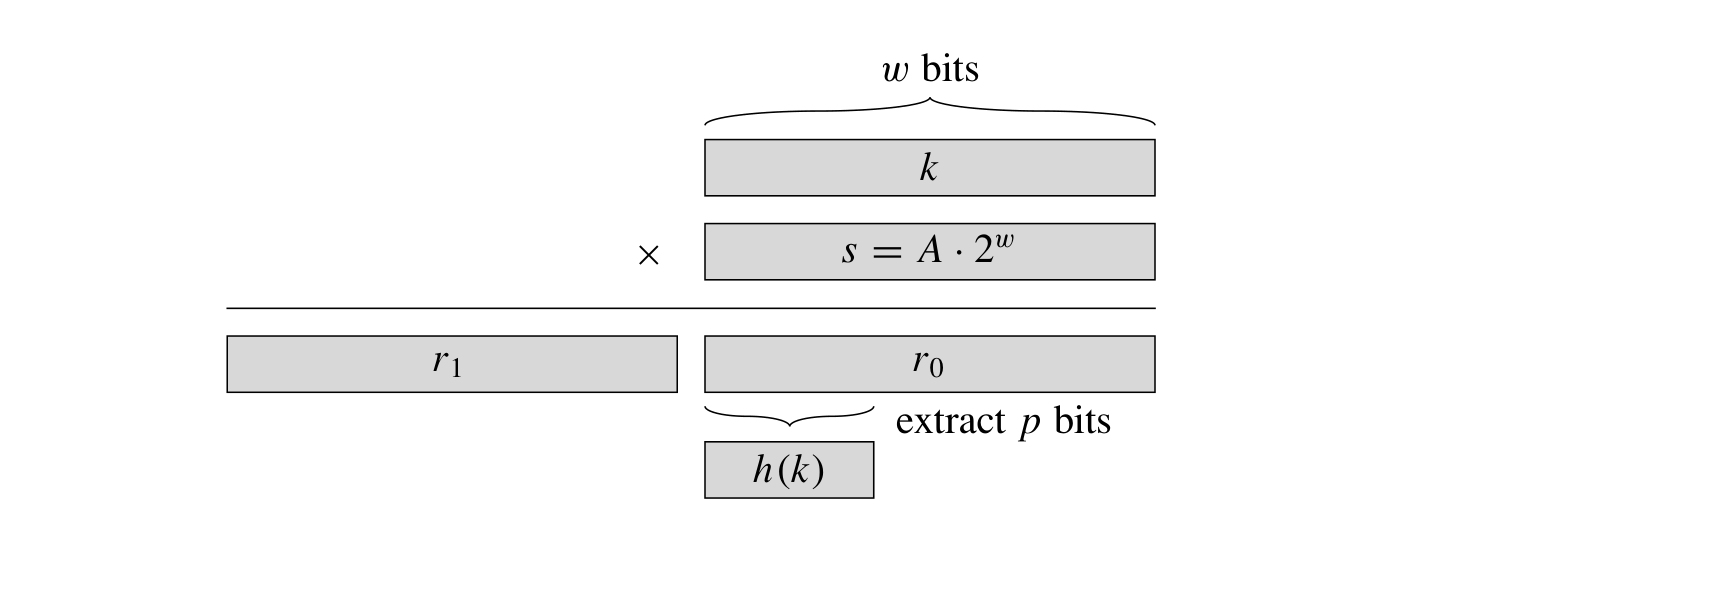
\includegraphics[width=\linewidth]{fig_11_4.png}

{\scriptsize\raggedright
\textbf{Como ler a figura:} a chave $k$ ocupa uma palavra de $w$ bits. Multiplica-se $k \cdot s$, com $s = \lfloor A\cdot 2^w \rfloor$, gerando um produto de $2w$ bits dividido em duas metades: a parte alta $r_1$ (descartada) e a parte baixa $r_0$, que representa $kA \bmod 1$ em ponto fixo. Os $p$ \alert{bits mais significativos} de $r_0$ são tomados como $h(k)$, equivalente a $\lfloor m\cdot(kA \bmod 1)\rfloor$ quando $m = 2^p$. Tudo se reduz a uma multiplicação e um \emph{shift}.\par}
\end{column}
\end{columns}
\end{frame}

\begin{frame}[shrink=15]{Exemplo numérico: método da multiplicação}
\textbf{Dados:} $k = 123\,456$, $m = 10\,000$, $A = (\sqrt{5}-1)/2 \approx 0{,}6180339887$.

\smallskip
\textbf{Passo 1.} Multiplique:
$$k\,A = 123\,456 \cdot 0{,}6180339887 \approx 76\,300{,}004115\ldots$$

\textbf{Passo 2.} Tome a parte fracionária:
$$k\,A \bmod 1 \approx 0{,}004115\ldots$$

\textbf{Passo 3.} Multiplique por $m$ e arredonde para baixo:
$$h(k) = \lfloor 10\,000 \cdot 0{,}004115\ldots \rfloor = \lfloor 41{,}15\ldots \rfloor = 41.$$

\smallskip
\textbf{Compare com a divisão:} $k \bmod 10\,000 = 3\,456$. Resultados \emph{muito} diferentes.

\smallskip
\begin{block}{Por que $A = (\sqrt 5 - 1)/2$?}
A razão áurea minimiza aglomerações de $\{kA \bmod 1\}_{k=1,2,\dots}$ no intervalo $[0,1)$ (teorema de Vera Sós sobre as três distâncias). Knuth: ``works reasonably well'' para qualquer chave.
\end{block}
\end{frame}

\begin{frame}{Hashing universal: defesa contra adversários}
\begin{itemize}
\item \textbf{Problema:} para qualquer função hash fixa, existe um conjunto de chaves que colide \emph{todas} no mesmo slot.
\item Um adversário malicioso pode forçar $\Theta(n)$ por operação.
\item \textbf{Ideia:} escolher $h$ \emph{aleatoriamente} de uma família $\mathcal H$ no início da execução.
\end{itemize}
\begin{block}{Família universal $\mathcal H$}
$\mathcal H$ é \emph{universal} se para cada par $k \neq \ell$,
$$\Pr_{h \in \mathcal H}[\,h(k) = h(\ell)\,] \le \frac{1}{m}.$$
\end{block}
Resultado: com $\mathcal H$ universal, a expectativa de busca cai para $\Theta(1 + \alpha)$ \emph{independentemente das chaves} escolhidas pelo adversário.
\end{frame}

\begin{frame}[shrink=5]{Uma família universal concreta (Carter--Wegman)}
\begin{block}{Construção}
Escolha um primo $p > \max(K)$. Para cada par $(a, b)$ com $a \in \{1, \dots, p-1\}$ e $b \in \{0, \dots, p-1\}$, defina
$$h_{a,b}(k) = ((a\,k + b) \bmod p) \bmod m.$$
A família $\mathcal H = \{h_{a,b}\}$ tem $p(p-1)$ funções e é \emph{universal}.
\end{block}
\textbf{Algoritmo:} ao iniciar a tabela, sorteie $a$ e $b$ uma única vez.

\smallskip
\textbf{Exemplo:} $p = 17$, $m = 6$, $a = 3$, $b = 4$.
\centering
\begin{tabular}{rcccc}
\toprule
$k$ & $a k + b$ & $\bmod\, 17$ & $\bmod\, 6$ & slot \\
\midrule
2  & $3\cdot 2 + 4 = 10$  & 10 & 4 & 4 \\
5  & $3\cdot 5 + 4 = 19$  & 2  & 2 & 2 \\
8  & $3\cdot 8 + 4 = 28$  & 11 & 5 & 5 \\
11 & $3\cdot 11 + 4 = 37$ & 3  & 3 & 3 \\
14 & $3\cdot 14 + 4 = 46$ & 12 & 0 & 0 \\
\bottomrule
\end{tabular}

\smallskip
Note que $28 = 1\cdot 17 + 11$, $37 = 2\cdot 17 + 3$, $46 = 2\cdot 17 + 12$. Sem aglomeração.

\smallskip
\textbf{Observação:} ataques reais (\emph{hash-flooding DoS}, 2003 e 2011) levaram Python, Ruby e Java a adotar hashes randomizados por padrão.
\end{frame}

%==============================================================
\section{Hashing de Strings}
%==============================================================

\begin{frame}[shrink=15]{Por que strings exigem cuidado especial?}
\begin{itemize}
\item Em quase toda aplicação real, as chaves são \emph{strings}: nomes, URLs, identificadores, sequências de DNA.
\item Uma string $s = s_0 s_1 \dots s_{L-1}$ é uma sequência de bytes (ou \emph{code units}). Como transformá-la num inteiro?
\item \alert{Tentação ingênua:} somar os códigos dos caracteres.
$$h(s) = \left(\sum_{i=0}^{L-1} s_i\right) \bmod m.$$
\item \textbf{Problema:} \texttt{"abc"}, \texttt{"bca"} e \texttt{"cab"} colidem (mesmos caracteres). Anagramas viram um campo minado.
\end{itemize}
\begin{alertblock}{Critério-chave}
Bom hash de strings tem que ser sensível à \emph{posição} de cada caractere, não só ao conjunto.
\end{alertblock}
\end{frame}

\begin{frame}[fragile]{Hash polinomial: a ideia central}
\textbf{Veja a string como os coeficientes de um polinômio em uma base $b$.}
$$h(s) = \big(s_0\, b^{L-1} + s_1\, b^{L-2} + \dots + s_{L-1}\, b^0\big) \bmod p.$$
\begin{itemize}
\item $b$ é uma base (tipicamente $31$, $33$, $37$, $131$ ou um primo).
\item $p$ é um primo grande ($\sim 10^9$) ou $2^{32}$ / $2^{64}$ (overflow natural).
\item Posições diferentes $\Rightarrow$ potências diferentes de $b$ $\Rightarrow$ anagramas não colidem.
\end{itemize}
\begin{block}{Avaliação eficiente (regra de Horner)}
$$h(s) = (\dots((s_0 \cdot b + s_1)\cdot b + s_2)\cdot b + \dots + s_{L-1}) \bmod p.$$
Custo: $L$ multiplicações e $L$ somas $\Rightarrow$ $\Theta(L)$.
\end{block}
\end{frame}

\begin{frame}[fragile]{Java: \texttt{String.hashCode()} e Python}
\textbf{Java} usa exatamente o hash polinomial com $b = 31$ e overflow em 32 bits:
\begin{verbatim}
public int hashCode() {
    int h = 0;
    for (int i = 0; i < length(); i++)
        h = 31 * h + charAt(i);
    return h;
}
\end{verbatim}
\begin{itemize}
\item Por que $31$? Primo ímpar; $31 \cdot h = (h \ll 5) - h$ (otimização clássica).
\item \alert{Cuidado:} \texttt{hashCode()} \emph{não é} o índice da tabela. \texttt{HashMap} aplica \texttt{(h \^{} (h >>> 16)) \& (m-1)} para misturar os bits altos.
\item \textbf{Python} (CPython) usa um polinômio com base $1000003$ e \emph{semente randomizada} a cada execução (defesa contra hash-flooding).
\end{itemize}
\end{frame}

\begin{frame}[fragile,shrink=10]{Exemplo numérico: $h(\texttt{"cat"})$ em Java}
\textbf{Caracteres:} \texttt{'c'} = 99, \texttt{'a'} = 97, \texttt{'t'} = 116. Base $b = 31$.

\smallskip
Aplicando Horner:
\begin{align*}
h_0 &= 0 \\
h_1 &= 31 \cdot 0 + 99 = 99 \\
h_2 &= 31 \cdot 99 + 97 = 3069 + 97 = 3166 \\
h_3 &= 31 \cdot 3166 + 116 = 98\,146 + 116 = 98\,262
\end{align*}

\medskip
Então \texttt{"cat".hashCode()} $= 98\,262$ (confere com a JVM).

\medskip
\textbf{Para uma tabela com $m = 16$ slots:} índice $= 98\,262 \bmod 16 = 6$.\\
{\footnotesize\textit{Verificação:} $98\,262 = 16 \cdot 6141 + 6 \Rightarrow$ resto $6$.}

\medskip
\textbf{Comparação:} \texttt{"act"} $\to 31\cdot(31\cdot 97 + 99) + 116 = 31\cdot 3106 + 116 = 96\,402$.\\
Slots diferentes. A ingênua soma daria $99 + 97 + 116 = 312$ para ambos.
\end{frame}

\begin{frame}{Hash rolante: o truque do Rabin--Karp}
\textbf{Problema:} encontrar um padrão $P$ (tamanho $L$) num texto $T$ (tamanho $n$).

\smallskip
\textbf{Ideia ingênua:} hashear cada subjanela de $T$ $\Rightarrow$ $\Theta(nL)$.

\smallskip
\textbf{Hash rolante:} se sabemos $h(T[i\,..\,i{+}L{-}1])$, conseguimos $h(T[i{+}1\,..\,i{+}L])$ em $O(1)$:
\begin{block}{Recorrência}
$$h_{i+1} = \big(b \cdot (h_i - T_i \cdot b^{L-1}) + T_{i+L}\big) \bmod p.$$
\end{block}
\begin{itemize}
\item Tirar o caractere mais antigo (multiplicado por $b^{L-1}$) e empurrar o novo.
\item Custo total da busca: $\Theta(n + L)$ esperado.
\item Em caso de \emph{match} de hash, comparamos as strings byte-a-byte para confirmar (defesa contra falso positivo).
\end{itemize}
\end{frame}

\begin{frame}[shrink=15]{Exemplo numérico: Rabin--Karp}
\textbf{Padrão:} $P = \texttt{"AB"}$ \quad \textbf{Texto:} $T = \texttt{"ABXAB"}$\\
Base $b = 256$, primo $p = 101$. Códigos: \texttt{A}=65, \texttt{B}=66, \texttt{X}=88.

\smallskip
\textbf{Hash do padrão:}
$$h(P) = (65 \cdot 256 + 66) \bmod 101 = 16\,706 \bmod 101.$$
$16\,706 = 165\cdot 101 + 41 \Rightarrow h(P) = 41.$

\smallskip
\textbf{Hash de $T[0..1] = \texttt{"AB"}$:} mesmo cálculo $\Rightarrow h_0 = 41$. \alert{Match!} Confirma byte-a-byte: \texttt{"AB"} = \texttt{"AB"} \checkmark.

\smallskip
\textbf{Roll para $T[1..2] = \texttt{"BX"}$:} ($b^{L-1} = 256$)
\begin{align*}
h_1 &= \big(256 \cdot (h_0 - 65 \cdot 256) + 88\big) \bmod 101 \\
    &= \big(256 \cdot (41 - 16\,640) + 88\big) \bmod 101.
\end{align*}
Trabalhando em $\bmod\, 101$: $256 \equiv 54$; $\ 65 \cdot 256 \equiv 65 \cdot 54 = 3510 \equiv 76$ (pois $34\cdot 101 = 3434$).\\
Então $h_1 \equiv 54 \cdot (41 - 76) + 88 \equiv 54 \cdot (-35) + 88 \equiv -1802 \equiv 16 \pmod{101}$.

\smallskip
\textit{Conferência direta:} $h(\texttt{"BX"}) = 66 \cdot 256 + 88 = 16\,984 \equiv 16 \pmod{101}$. \checkmark

\smallskip
\textbf{Próximo roll $\to T[2..3]=\texttt{"XA"}$, depois $T[3..4]=\texttt{"AB"}$:} hash voltará a $41 \Rightarrow$ segundo match (confirmado byte-a-byte).
\end{frame}

\begin{frame}[fragile]{Hashes não-criptográficos modernos: panorama}
\begin{itemize}
\item \textbf{DJB2} (Daniel J.\ Bernstein, 1991):
\begin{verbatim}
unsigned long h = 5381;
while ((c = *s++))
    h = ((h << 5) + h) + c;   // h * 33 + c
\end{verbatim}
Simples, rápido, popular em código C clássico.

\item \textbf{FNV-1a:} multiplicação por primo grande + XOR. Ainda usado em \texttt{powershell}, \texttt{sqlite}, redes.

\item \textbf{MurmurHash3} (Austin Appleby, 2008): pipeline de \emph{mix} (multiplicação, rotação, XOR). Padrão em Hadoop, Cassandra, Redis.

\item \textbf{CityHash / FarmHash} (Google) e \textbf{xxHash}: explora SIMD; $> 10$ GB/s.

\item \textbf{SipHash} (Aumasson--Bernstein, 2012): \emph{criptograficamente seguro} e rápido; adotado em Python, Ruby, Rust após os ataques de hash-flooding.
\end{itemize}
\end{frame}

\begin{frame}[shrink=15]{Exemplo numérico: DJB2 sobre \texttt{"cat"}}
DJB2: $h \gets 5381$; \  para cada char $c$: \ $h \gets 33\,h + c$. Todas as contas em $\mathbb{Z}_{2^{32}}$ (aqui ignoramos overflow porque o valor cabe em 32 bits).

\smallskip
\centering
\begin{tabular}{lrll}
\toprule
Passo & $h$ atual & Operação & Novo $h$ \\
\midrule
início       & $5\,381$       & ---                              & $5\,381$ \\
ler \texttt{c} (99)   & $5\,381$       & $33 \cdot 5\,381 + 99 = 177\,573 + 99$    & $177\,672$ \\
ler \texttt{a} (97)   & $177\,672$     & $33 \cdot 177\,672 + 97 = 5\,863\,176 + 97$ & $5\,863\,273$ \\
ler \texttt{t} (116)  & $5\,863\,273$  & $33 \cdot 5\,863\,273 + 116$              & $193\,488\,125$ \\
\bottomrule
\end{tabular}

\smallskip
\textbf{Verificações:}
$33 \cdot 5\,381 = 32 \cdot 5\,381 + 5\,381 = 172\,192 + 5\,381 = 177\,573$.\\
$33 \cdot 177\,672 = 32 \cdot 177\,672 + 177\,672 = 5\,685\,504 + 177\,672 = 5\,863\,176$.\\
$33 \cdot 5\,863\,273 = 5\,863\,273 \cdot 32 + 5\,863\,273 = 187\,624\,736 + 5\,863\,273 = 193\,488\,009$; \  $+116 = 193\,488\,125$.

\smallskip
\textbf{Compare com Java:} para \texttt{"cat"}, Java $=98\,262$, DJB2 $=193\,488\,125$. Mesma string, ``digital'' totalmente diferente.
\end{frame}

\begin{frame}{Hashing duplo para strings: robustez extra}
\begin{itemize}
\item Mesmo um bom hash de string pode colidir por azar quando aplicamos $\bmod\,p$.
\item \textbf{Truque competitivo (programação competitiva, bioinformática):} calcule \emph{dois} hashes independentes
$$H(s) = \big(h_{p_1, b_1}(s),\; h_{p_2, b_2}(s)\big)$$
com primos $p_1, p_2$ distintos e bases $b_1, b_2$.
\item Duas strings só são consideradas iguais se \emph{ambos} os hashes baterem.
\item Probabilidade de falso positivo: $\approx 1/(p_1 p_2) \approx 10^{-18}$.
\item Útil em: comparação de substrings de DNA, \emph{longest common substring}, deduplicação em larga escala.
\end{itemize}
\end{frame}

%==============================================================
\section{Endereçamento Aberto}
%==============================================================

\begin{frame}{Definição: endereçamento aberto}
\begin{block}{Definição: endereçamento aberto}
Um esquema de resolução de colisões em que \alert{todas as chaves são armazenadas na própria tabela $T[0\dots m-1]$}, sem listas ou estruturas auxiliares. Para cada chave $k$, define-se uma \alert{sequência de sondagem}
$$\langle h(k,0),\; h(k,1),\; \dots,\; h(k,m-1) \rangle,$$
uma \emph{permutação} de $\{0,1,\dots,m-1\}$. Para inserir/buscar, percorre-se essa sequência até encontrar o slot da chave (ou um slot vazio).
\end{block}
\begin{itemize}
\item Restrição estrutural: $n \le m$ (não há onde guardar mais chaves que slots).
\item Vantagens: sem ponteiros, melhor uso de cache, menor consumo de memória.
\item Custo: remoção exige cuidado (marcadores \emph{DELETED}) e desempenho degrada quando $\alpha \to 1$.
\end{itemize}
\end{frame}

\begin{frame}{Endereçamento aberto: sem listas externas}
\begin{itemize}
\item Todos os elementos ficam \emph{dentro} da tabela: $n \le m$.
\item Quando $T[h(k)]$ está ocupado, tentamos $T[h_1(k)], T[h_2(k)], \dots$ até achar slot vazio.
\item Definimos $h : U \times \{0,1,\dots,m-1\} \to \{0,1,\dots,m-1\}$ tal que
$$\langle h(k,0), h(k,1), \dots, h(k,m-1) \rangle$$
é uma \emph{permutação} de $\{0,\dots,m-1\}$.
\item Inserção tenta a sequência de \emph{sondagem} até encontrar vazio.
\end{itemize}
\end{frame}

\begin{frame}{Motivação: sondagem linear}
\textbf{Ideia intuitiva:} se o slot $h'(k)$ está ocupado, \emph{olhe o próximo}, depois o seguinte, e assim por diante -- como procurar uma vaga andando em linha reta pelo estacionamento.
\begin{block}{Sondagem linear}
$$h(k,i) = (h'(k) + i) \bmod m, \quad i = 0, 1, \dots, m-1.$$
\end{block}
\begin{itemize}
\item \alert{Prós:} simples de implementar; ótimo para a \emph{cache} (acessos sequenciais).
\item \alert{Contra:} sofre de \emph{aglomeração primária} -- uma vez formado um cluster, ele cresce ainda mais rápido (chaves que caem em qualquer slot do cluster o estendem).
\item Apenas $m$ sequências de sondagem distintas (uma por slot inicial).
\end{itemize}
\end{frame}

\begin{frame}{Motivação: sondagem quadrática}
\textbf{Problema da linear:} clusters contíguos. \textbf{Solução:} \emph{saltos crescentes} em vez de passos unitários, espalhando a sondagem pela tabela.
\begin{block}{Sondagem quadrática}
$$h(k,i) = (h'(k) + c_1 i + c_2 i^2) \bmod m, \quad c_2 \neq 0.$$
\end{block}
\begin{itemize}
\item \alert{Prós:} elimina a aglomeração primária; passos $1, 4, 9, 16, \dots$ pulam clusters.
\item \alert{Contra:} \emph{aglomeração secundária} -- duas chaves com mesmo $h'(k)$ percorrem \emph{a mesma} sequência.
\item Ainda $m$ sequências distintas; $c_1, c_2, m$ precisam ser escolhidos para a sequência cobrir toda a tabela.
\end{itemize}
\end{frame}

\begin{frame}{Motivação: duplo hashing}
\textbf{Problema das duas anteriores:} o \emph{passo} de sondagem depende só de $h'(k)$. \textbf{Ideia:} usar uma \emph{segunda função hash} para que o passo dependa da própria chave.
\begin{block}{Duplo hashing}
$$h(k,i) = (h_1(k) + i\, h_2(k)) \bmod m.$$
\end{block}
\begin{itemize}
\item \alert{Prós:} chaves distintas com mesmo $h_1$ usam passos diferentes $\Rightarrow$ elimina aglomeração secundária.
\item Gera $\Theta(m^2)$ sequências de sondagem distintas (aproxima o ideal de \emph{hashing uniforme}).
\item \alert{Requisito:} $h_2(k)$ deve ser \emph{coprimo} com $m$ (ex.: $m$ primo, ou $m = 2^p$ com $h_2$ ímpar) para a sequência ser uma permutação.
\end{itemize}
\end{frame}

\begin{frame}{Sondagem linear: visualizando o \emph{cluster}}
\centering
\begin{tikzpicture}[scale=0.85, every node/.style={font=\small},
  rowlabel/.style={anchor=east, font=\footnotesize}]
% header
\node[rowlabel] at (-0.7, 0.5) {Slot:};
\foreach \i in {0,...,9}{
  \node at (\i, 0.5) {\i};
}
% empty row initially
\foreach \i in {0,...,9}{
  \draw (\i-0.5, -0.5) rectangle (\i+0.5, 0);
}
\node[rowlabel] at (-0.7,-0.25) {Inicial};

% step: inserts h(k)=3, then 3 again, then 4...
\foreach \i in {0,...,9}{
  \draw (\i-0.5, -1.5) rectangle (\i+0.5, -1);
}
\node[fill=slotOcup, rectangle, draw, minimum width=0.95cm, minimum height=0.45cm] at (3, -1.25) {$k_1$};
\node[rowlabel] at (-0.7,-1.25) {Insere $k_1$ ($h=3$)};

\foreach \i in {0,...,9}{
  \draw (\i-0.5, -2.5) rectangle (\i+0.5, -2);
}
\node[fill=slotOcup, rectangle, draw, minimum width=0.95cm, minimum height=0.45cm] at (3, -2.25) {$k_1$};
\node[fill=slotColisao, rectangle, draw, minimum width=0.95cm, minimum height=0.45cm] at (4, -2.25) {$k_2$};
\node[rowlabel] at (-0.7,-2.25) {Insere $k_2$ ($h=3$, sonda 4)};

\foreach \i in {0,...,9}{
  \draw (\i-0.5, -3.5) rectangle (\i+0.5, -3);
}
\node[fill=slotOcup, rectangle, draw, minimum width=0.95cm, minimum height=0.45cm] at (3, -3.25) {$k_1$};
\node[fill=slotColisao, rectangle, draw, minimum width=0.95cm, minimum height=0.45cm] at (4, -3.25) {$k_2$};
\node[fill=slotColisao, rectangle, draw, minimum width=0.95cm, minimum height=0.45cm] at (5, -3.25) {$k_3$};
\node[rowlabel] at (-0.7,-3.25) {Insere $k_3$ ($h=4$, sonda 5)};

\draw[decorate, decoration={brace, amplitude=4pt, mirror}] (2.5,-3.7) -- (5.5,-3.7) node[midway, below=4pt] {\footnotesize cluster};
\end{tikzpicture}

\vspace{0.2cm}
{\small Sondagem linear cria \emph{aglomerados}: uma colisão atrai novas colisões.}
\end{frame}

\begin{frame}[shrink=20]{Exemplo: busca em tabela com sondagem linear}
\textbf{Tabela $m = 11$, $h(k) = k \bmod 11$.} Estado atual:

\smallskip
\centering
\begin{tabular}{c|c|c|c|c|c|c|c|c|c|c}
0 & 1 & 2 & 3 & 4 & 5 & 6 & 7 & 8 & 9 & 10 \\
\hline
22 & 88 & -- & 14 & 25 & 36 & 47 & -- & -- & 9 & -- \\
\end{tabular}

\smallskip
\textbf{Buscar $k = 36$:}
\begin{itemize}
\item Sonda 0: $h(36) = 36 \bmod 11 = 3$. $T[3] = 14 \neq 36$. \alert{Continua.}
\item Sonda 1: $T[4] = 25 \neq 36$. \alert{Continua.}
\item Sonda 2: $T[5] = 36$. \textbf{Achou!} Custo: 3 acessos.
\end{itemize}

\textbf{Buscar $k = 100$ (ausente):}
\begin{itemize}
\item $h(100) = 100 \bmod 11 = 1$. Sondas: $T[1]=88, T[2]=$ vazio $\Rightarrow$ \textbf{não está}.
\end{itemize}

\begin{alertblock}{Por que slot vazio termina a busca}
Em endereçamento aberto sem remoções, encontrar vazio $\Rightarrow$ chave nunca foi inserida (caso contrário, ela teria parado aqui). Remoções exigem marcador \textsc{deleted} para preservar a invariante.
\end{alertblock}
\end{frame}

\begin{frame}{Duplo hashing em ação}
\begin{columns}[T]
\begin{column}{0.45\textwidth}
\begin{itemize}
\item Tabela de tamanho $m = 13$.
\item $h_1(k) = k \bmod 13$
\item $h_2(k) = 1 + (k \bmod 11)$
\item Inserção (nessa ordem): $79, 69, 72, 98, 14, 50$.
\item Cada chave usa um \emph{passo} diferente, evitando aglomerados.
\end{itemize}
\end{column}
\begin{column}{0.50\textwidth}
\centering
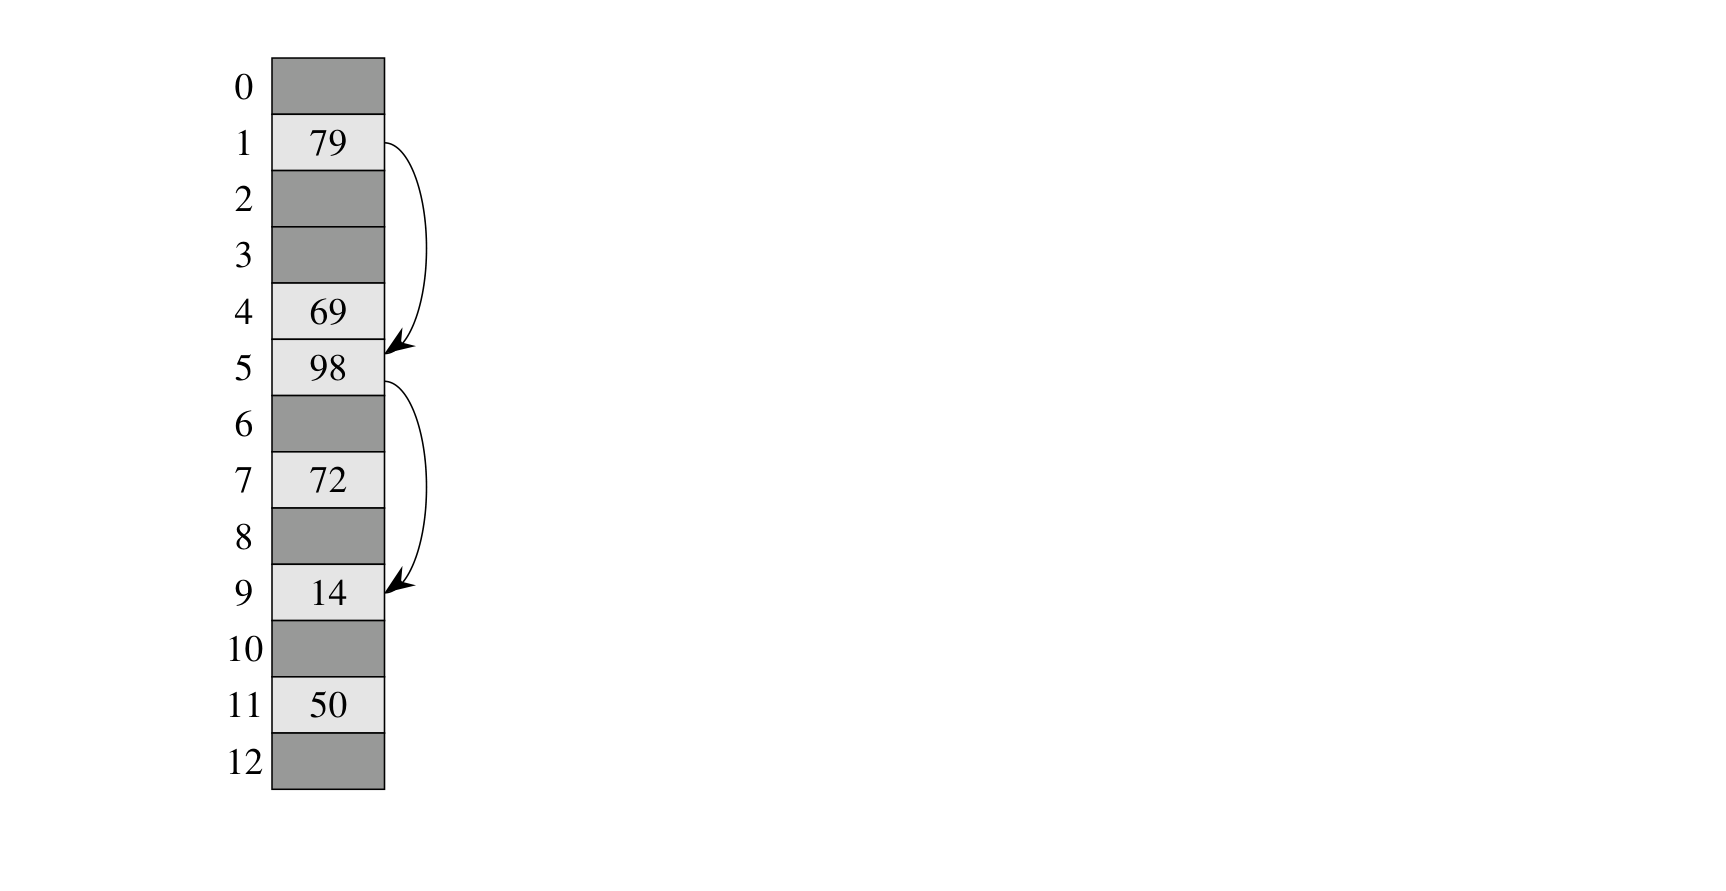
\includegraphics[width=\linewidth]{fig_11_5.png}
{\scriptsize Estado da tabela após as inserções.}
\end{column}
\end{columns}
\end{frame}

\begin{frame}[shrink=15]{Traço passo a passo do duplo hashing}
$h_1(k) = k \bmod 13$, $h_2(k) = 1 + (k \bmod 11)$, $h(k,i) = (h_1 + i\cdot h_2) \bmod 13$.

\smallskip
\centering
\begin{tabular}{rrrll}
\toprule
$k$ & $h_1$ & $h_2$ & Sequência de sondagem & Slot final \\
\midrule
79 & 1 & $1+2=3$ & $1$ & 1 \\
69 & 4 & $1+3=4$ & $4$ & 4 \\
72 & 7 & $1+6=7$ & $7$ & 7 \\
98 & 7 & $1+10=11$ & $7$ (ocup.\ por 72), $(7+11)\bmod 13 = 5$ & 5 \\
14 & 1 & $1+3=4$ & $1$ (ocup.), $(1+4)=5$ (ocup.), $(1+8)=9$ & 9 \\
50 & 11 & $1+6=7$ & $11$ & 11 \\
\bottomrule
\end{tabular}

\smallskip
\textbf{Verificações:}
$79 \bmod 13 = 79 - 6\cdot 13 = 79 - 78 = 1$.\ \  $98 \bmod 13 = 98 - 7\cdot 13 = 98 - 91 = 7$.\\
$98 \bmod 11 = 98 - 8\cdot 11 = 98 - 88 = 10$.\ \  $50 \bmod 13 = 50 - 3\cdot 13 = 50 - 39 = 11$.

\smallskip
Estado final coincide com a Fig.\ 11.5: slots $1, 4, 5, 7, 9, 11$ ocupados.
\end{frame}

\begin{frame}[shrink=15]{Análise do endereçamento aberto}
\textbf{Hipótese de hashing uniforme:} cada chave tem como sequência de sondagem qualquer permutação de $\{0,\dots,m-1\}$ com igual probabilidade.

\begin{block}{Resultados (fator de carga $\alpha = n/m < 1$)}
\begin{itemize}
\item Busca \emph{sem sucesso}: em média $\le \dfrac{1}{1-\alpha}$ sondagens.
\item Busca \emph{com sucesso}: em média $\le \dfrac{1}{\alpha}\ln\dfrac{1}{1-\alpha}$ sondagens.
\end{itemize}
\end{block}

\centering
\begin{tabular}{ccc}
\toprule
$\alpha$ & Busca sem sucesso & Busca com sucesso \\
\midrule
$0{,}5$ & $\approx 2{,}0$ & $\approx 1{,}39$ \\
$0{,}9$ & $\approx 10{,}0$ & $\approx 2{,}56$ \\
$0{,}99$ & $\approx 100$ & $\approx 4{,}65$ \\
\bottomrule
\end{tabular}

\vspace{0.2cm}
\textbf{Mensagem:} mantenha $\alpha$ longe de 1 (tipicamente $\le 0{,}75$).
\end{frame}

%==============================================================
\section{Hashing Perfeito}
%==============================================================

\begin{frame}{Definição: hashing perfeito}
\begin{block}{Definição: hash perfeito}
Dado um conjunto \alert{estático} de chaves $K = \{k_1, k_2, \dots, k_n\}$, uma função hash $h: U \to \{0, 1, \dots, m-1\}$ é dita \emph{perfeita} para $K$ se ela é \alert{injetiva} sobre $K$ -- isto é, para todo $k_i, k_j \in K$ com $k_i \neq k_j$, vale $h(k_i) \neq h(k_j)$.
\end{block}
\begin{itemize}
\item Sem colisões em $K$ $\Rightarrow$ busca em $O(1)$ \alert{no pior caso}.
\item Se, além disso, $m = n$, $h$ é dita \alert{mínima} (sem slots vazios).
\item Construção é viável porque $K$ é conhecido em tempo de projeto.
\end{itemize}
\end{frame}

\begin{frame}{Hashing perfeito: $O(1)$ \emph{no pior caso}}
\begin{itemize}
\item Aplicável quando o conjunto de chaves $K$ é \alert{estático} (conhecido em tempo de projeto).
\item Exemplos: palavras-chave de uma linguagem de programação, símbolos de um arquivo de objeto.
\item Objetivo: garantir que a busca custe $O(1)$ \emph{no pior caso}.
\end{itemize}
\begin{block}{Estratégia em dois níveis}
\begin{enumerate}
\item Hash primário $h$ distribui as $n$ chaves em $m = n$ slots.
\item Cada slot $j$ com $n_j$ chaves tem uma sub-tabela $S_j$ de tamanho $m_j = n_j^2$, com função $h_j$ escolhida para não ter colisões.
\end{enumerate}
\end{block}
\end{frame}

\begin{frame}{Esquema de dois níveis}
\centering
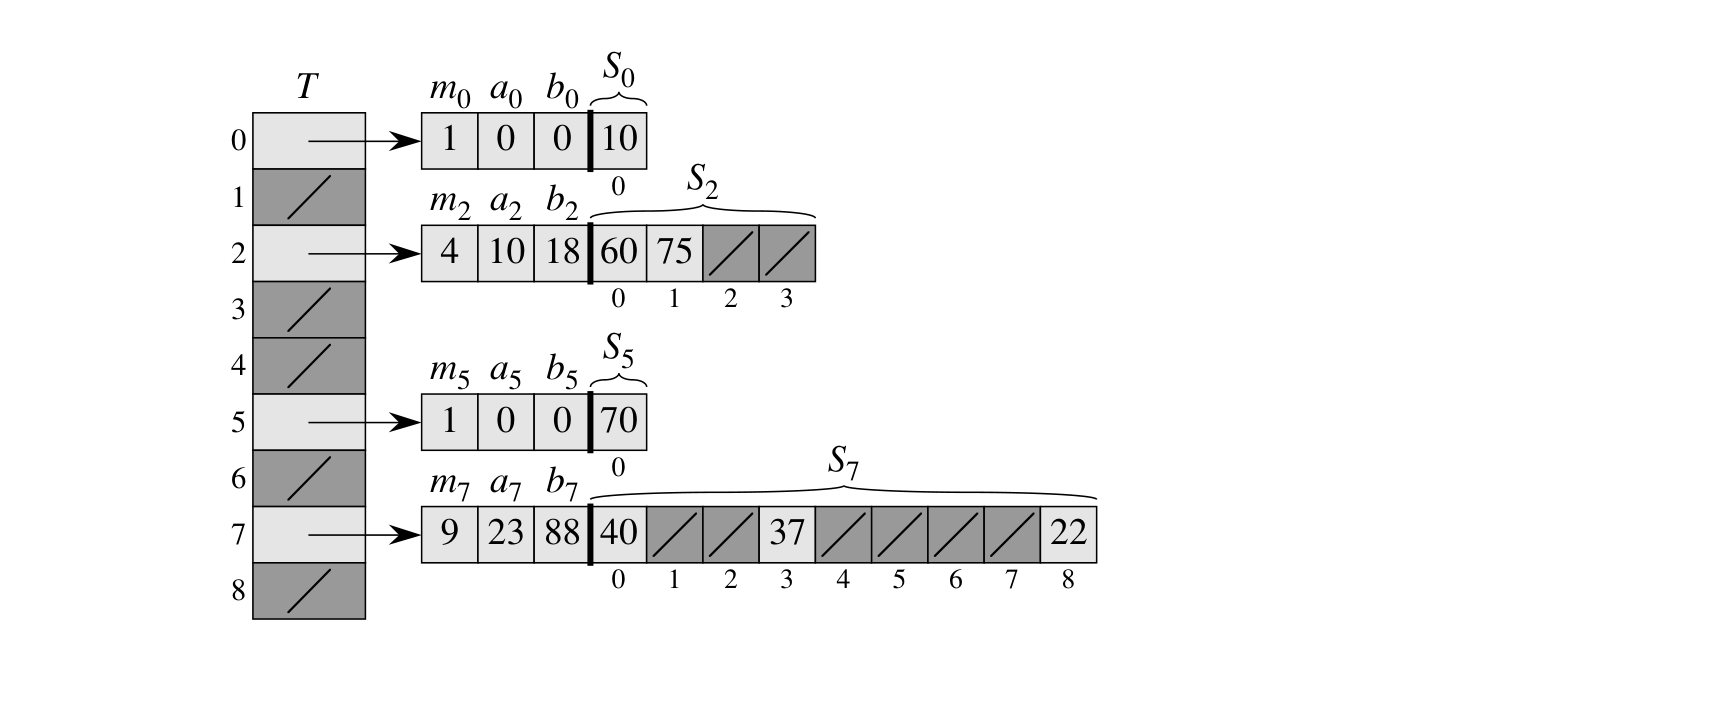
\includegraphics[width=0.62\linewidth]{fig_11_6.png}

{\scriptsize Hashing perfeito armazenando $K = \{10, 22, 37, 40, 60, 70, 75\}$.}

\medskip
\begin{itemize}\scriptsize
\item \alert{Tabela primária $T$}: hash $h(k) = ((a\,k + b) \bmod p) \bmod m$ distribui as $n=7$ chaves em $m=9$ slots; cada slot $j$ guarda os parâmetros $(m_j, a_j, b_j)$ da sub-tabela.
\item \alert{Sub-tabelas $S_j$}: tamanho $m_j = n_j^2$ (ex.: slot 2 tem $n_2 = 2$ chaves $\Rightarrow m_2 = 4$); a função $h_j$ é escolhida até não haver colisão.
\item Slots vazios ($n_j = 0$) não alocam sub-tabela; a busca por $k$ faz \emph{dois} acessos: $T[h(k)]$ e $S_{h(k)}[h_{h(k)}(k)]$.
\end{itemize}
\end{frame}

\begin{frame}{Por que $m_j = n_j^2$ funciona?}
\textbf{Teorema 11.9:} se armazenamos $n$ chaves em uma tabela de tamanho $m = n^2$ com $h$ escolhida \emph{aleatoriamente} de uma família universal, a probabilidade de haver alguma colisão é $< 1/2$.

\medskip
\textbf{Consequência:} basta tentar algumas funções $h_j$ até encontrar uma sem colisões em cada sub-tabela.

\begin{block}{Espaço total}
$$E\!\left[\sum_{j=0}^{m-1} n_j^2\right] < 2n.$$
Ou seja, em média gastamos $O(n)$ de espaço para garantir $O(1)$ de busca \emph{no pior caso}.
\end{block}
\end{frame}

%==============================================================
\section{Síntese}
%==============================================================

\begin{frame}{Quando usar cada esquema?}
\centering
\begin{tabular}{p{4cm}p{4.5cm}p{4cm}}
\toprule
\textbf{Cenário} & \textbf{Estrutura recomendada} & \textbf{Porquê} \\
\midrule
Universo pequeno e denso & Endereçamento direto & $O(1)$ trivial, sem hash. \\
Conjunto dinâmico, $\alpha$ pode crescer & Encadeamento & Tolera $\alpha > 1$. \\
Memória limitada, $\alpha < 0{,}75$ & Endereçamento aberto (duplo hashing) & Sem ponteiros, cache-friendly. \\
Conjunto estático, busca crítica & Hashing perfeito & $O(1)$ no pior caso. \\
Adversário malicioso & Família universal de hashes & Independência das chaves. \\
\bottomrule
\end{tabular}
\end{frame}

\begin{frame}{Pontos-chave para levar para casa}
\begin{itemize}
\item Tabelas hash transformam $\Theta(\log n)$ ou $\Theta(n)$ em $\Theta(1)$ \emph{esperado}.
\item Função hash boa $=$ rápida $+$ bem distribuída.
\item \alert{Sempre há colisões} -- a engenharia está em como tratá-las.
\item Fator de carga $\alpha = n/m$ é o parâmetro mestre da análise.
\item Para garantias contra adversários: \emph{universal hashing}.
\item Para $O(1)$ no pior caso (chaves estáticas): \emph{hashing perfeito}.
\end{itemize}
\end{frame}

\begin{frame}{Exercícios sugeridos}
\setbeamercolor{block title}{bg=exercicio,fg=black}
\begin{block}{1. Aglomeração}
Insira as chaves $10, 22, 31, 4, 15, 28, 17, 88, 59$ em uma tabela de tamanho $m=11$ usando:
\begin{enumerate}
\item encadeamento com $h(k) = k \bmod 11$;
\item sondagem linear com o mesmo $h$;
\item duplo hashing com $h_2(k) = 1 + (k \bmod 10)$.
\end{enumerate}
Compare os números de sondagens.
\end{block}
\begin{block}{2. Fator de carga}
Mostre que, sob hashing uniforme simples e encadeamento, a busca sem sucesso custa $\Theta(1+\alpha)$ em média.
\end{block}
\end{frame}

\begin{frame}{Referências}
\begin{itemize}
\item Cormen, T.\ H.; Leiserson, C.\ E.; Rivest, R.\ L.; Stein, C. \emph{Introduction to Algorithms}. 2.ed. MIT Press, 2001. \textbf{Capítulo 11 -- Hash Tables.}
\item Knuth, D.\ E. \emph{The Art of Computer Programming, Vol.\ 3: Sorting and Searching.} 2.ed. Addison-Wesley, 1998. \textbf{Seções 6.4.}
\item Carter, J.\ L.; Wegman, M.\ N. ``Universal classes of hash functions.'' \emph{Journal of Computer and System Sciences}, 18(2):143--154, 1979.
\end{itemize}
\vfill
{\scriptsize Figuras 11.1--11.6 extraídas da edição 2001 do Cormen \emph{et al.} para fins educacionais.}
\end{frame}

\end{document}
